\subsection{Scenario of Use}
\label{subsec:scenario}
%In this section, an example of the application of our approach to a software development project is described.

The scenario describes a software development project. It contains $12$ files arranged hierarchically as depicted by the file tree in Figure \ref{fig_fileTreeExample}. 

\begin{figure}
	\centering
	\scriptsize{
	\begin{forest}
%		for tree={
%			font=\ttfamily,
%			grow'=0,
%			child anchor=west,
%			parent anchor=south,
%			anchor=west,
%			calign=first,
%			inner xsep=10pt,
%			edge path={
%				\noexpand\path [draw, \forestoption{edge}]
%				(!u.south west) +(7.5pt,0) |- node[fill,inner sep=1.25pt] {} (.child anchor)\forestoption{edge label};
%			},
%			before typesetting nodes={
%				if n=1
%				{insert before={[,phantom]}}
%				{}
%			},
%			fit=band,
%			before computing xy={l=15pt},
%		}  
		[StoryMiningSoftwareRepositories ($f_1$)
			[README.md ($f_2$)]
			[running example ($f_3$)
				[Requirements ($f_4$)
					[requirements.txt ($f_5$)]
				]
				[Software ($f_6$)
					[model.java ($f_7$)]
					[test.java ($f_8$)]
					[packages ($f_9$) [
						p1 ($f_{10}$)
							[visualization.txt ($f_{11}$)] 
						]
					]
				]
				[specification.txt ($f_{12}$)]
			]
		]
	\end{forest}
	}
	\caption{File tree describing the file structure in our scenario of use.}
	\label{fig_fileTreeExample}
\end{figure}

At the first level of the file tree there is the README.md file. This is typically used to describe the project. The software product in our case is called \emph{running example} and is contained in the $f_5$. The product consists of an example for software developers who want to organize their projects according to a predefined structure. 

%There are several resources  that collaborate in the project. Their roles are shown in \Cref{tab:resource-roles}. According to the role, each resource has a typical scope on the project, e.g., \emph{John} is the project manager and can work on all the project, \emph{Mary} is a graphic designer and she can only work on the visualization. 
%
%\begin{table}[]
\centering
\caption{Role and scope of the resources in our scenario of use.}
\label{tab:resource-roles}
\begin{tabular}{@{}llll@{}}
\toprule
 Id &Resouce & Role                  & Scope        \\  \midrule
u1 & Anna     & Software developer    & Software     \\
u2 &Beth     & Software developer    & Software     \\
u3 &Dom      & Tester                & Software     \\
u4 &Earl     & Tester                & Software     \\
u5 &John     & Project manager       & Project      \\
u6 &Mary     & Graphic designer      & p1           \\
u7 &Mark     & Requirements engineer & Requirements \\
u8 &Paul     & Requirements engineer & Requirements \\ \bottomrule
\end{tabular}
\end{table}

The software development project has 21 commits, which check in changes happened over 10 days. Table \ref{tab:vcs-log-data} illustrates an excerpt from the VCS log of this scenario of use. The project managers are interested in understanding the work process done by project participants in each of the files and whether there is some dependency between them that may emerge from the data. We now show how our approach can fulfill this requirements, by applying  each step of our approach to this project example and discussing the outcomes.





%\begin{figure}
%\centering
%
\includegraphics[scale=0.5]{figures/Containments}
%\caption{Structure of the project.}
%\label{fig:Containments}
%\end{figure}


%As described in Section \ref{} the first step of the approach is the generation of file process considering story mining techniques. Based on the comments presented in Table \ref{} the process for all four files were generated. Next the method to extract dependencies between files is run. For that the time series with the amount of change for each file is generated. Considering the correlation between the files the dependencies are found. Figure \ref{} depicts the proposed visualization of the 3 perspectives of a file.   
%
%%\onecolumn{
%\begin{figure*}[t]
%\centering
%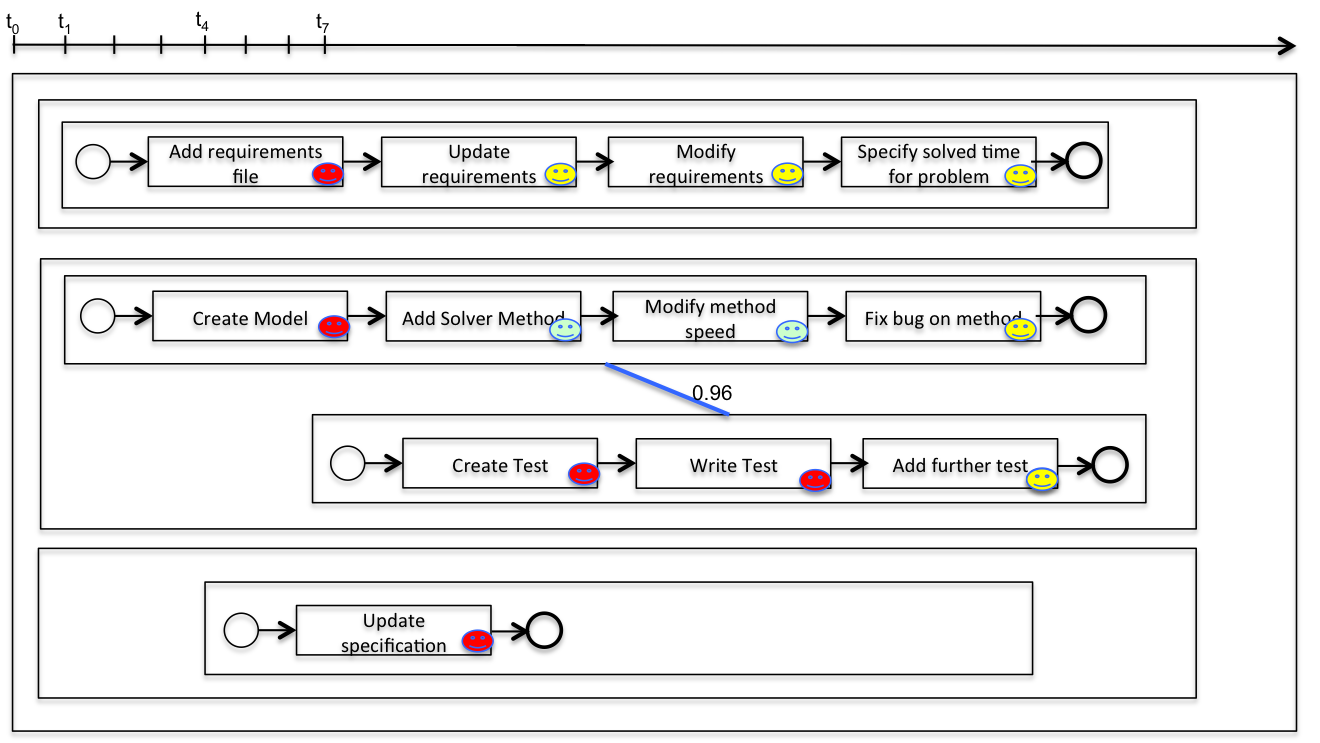
\includegraphics[scale=0.8]{figures/ExampleProposedVisualization}
%\caption{Illustration of the proposed visualization.}
%\label{fig:Containments}
%\end{figure*}
%%}

%ToDo
%Figure with the containments
%Table with the commits (junction of the .xls files. Consider only the amount of change. Express time by $t_i$
%Figure with the containments instanciated with the file processes and the dependencies.